\documentclass[tikz]{standalone}
\usepackage[utf8]{inputenc}
\usepackage{amsmath}
\usetikzlibrary{calc,shadows}

\definecolor{mycolor}{RGB}{12,18,33}

\begin{document}
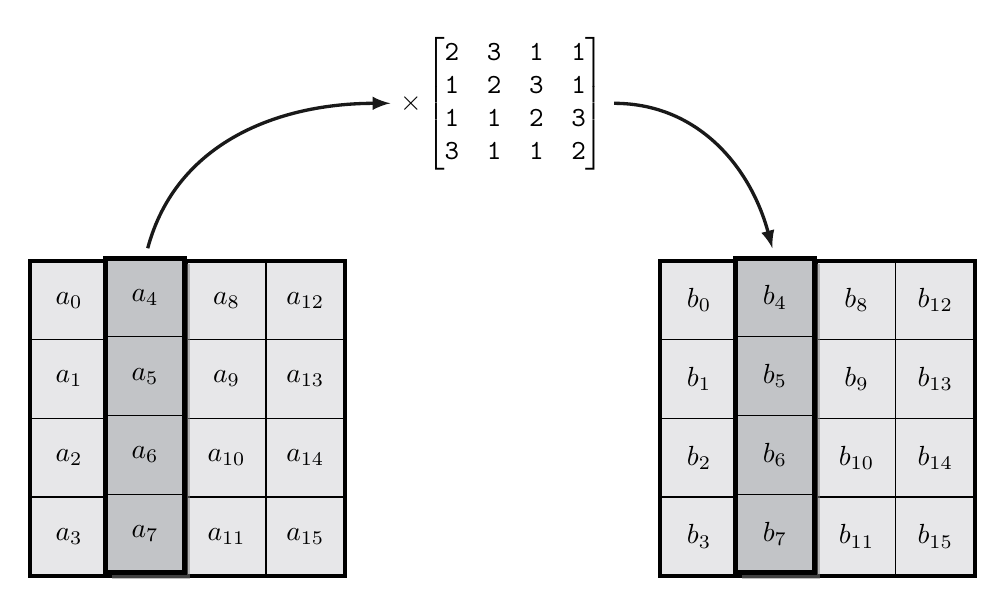
\begin{tikzpicture}
% state before
\foreach\x in {0, 1, ..., 3}
\foreach\y in {0, 1, ..., 3}
\draw[fill=mycolor!10] (\x,\y) rectangle ($(\x,\y) + (1, 1)$);

\draw[line width=1.5pt] (0,0) rectangle (4,4);

% slightly shifted column
\draw[line width=1.8pt,drop shadow,fill=mycolor!25,shift={(-1pt,1pt)}] (1,0) rectangle (2,4);
\node[shift={(-1pt,1pt)}] at (1.5, 0.5) {$a_7$};
\node[shift={(-1pt,1pt)}] at (1.5, 1.5) {$a_6$};
\node[shift={(-1pt,1pt)}] at (1.5, 2.5) {$a_5$};
\node[shift={(-1pt,1pt)}] at (1.5, 3.5) {$a_4$};
\foreach\y in {1, 2, 3}
\draw[shift={(-1pt,1pt)}] (1,\y) --++ (1,0);

\node at (0.5, 0.5) {$a_3$};
\node at (0.5, 1.5) {$a_2$};
\node at (0.5, 2.5) {$a_1$};
\node at (0.5, 3.5) {$a_0$};
\node at (2.5, 0.5) {$a_{11}$};
\node at (2.5, 1.5) {$a_{10}$};
\node at (2.5, 3.5) {$a_8$};
\node at (2.5, 2.5) {$a_9$};
\node at (3.5, 0.5) {$a_{15}$};
\node at (3.5, 1.5) {$a_{14}$};
\node at (3.5, 2.5) {$a_{13}$};
\node at (3.5, 3.5) {$a_{12}$};

\node[shift={(-1pt,1pt)}] (a) at (1.5,4) {};

% state after
\begin{scope}[shift={(8,0)}]

\foreach\x in {0, 1, ..., 3}
\foreach\y in {0, 1, ..., 3}
\draw[fill=mycolor!10] (\x, \y) rectangle ($(\x, \y) + (1, 1)$);

\draw[line width=1.5pt] (0, 0) rectangle (4,4);

% slightly shifted column
\draw[line width=1.8pt,drop shadow,fill=mycolor!25,shift={(-1pt,1pt)}] (1,0) rectangle (2,4);
\node[shift={(-1pt,1pt)}] at (1.5, 0.5) {$b_7$};
\node[shift={(-1pt,1pt)}] at (1.5, 1.5) {$b_6$};
\node[shift={(-1pt,1pt)}] at (1.5, 2.5) {$b_5$};
\node[shift={(-1pt,1pt)}] at (1.5, 3.5) {$b_4$};
\foreach\y in {1, 2, 3}
\draw[shift={(-1pt,1pt)}] (1,\y) --++ (1,0);

\node at (0.5, 0.5) {$b_3$};
\node at (0.5, 1.5) {$b_2$};
\node at (0.5, 2.5) {$b_1$};
\node at (0.5, 3.5) {$b_0$};
\node at (2.5, 0.5) {$b_{11}$};
\node at (2.5, 1.5) {$b_{10}$};
\node at (2.5, 3.5) {$b_8$};
\node at (2.5, 2.5) {$b_9$};
\node at (3.5, 0.5) {$b_{15}$};
\node at (3.5, 1.5) {$b_{14}$};
\node at (3.5, 2.5) {$b_{13}$};
\node at (3.5, 3.5) {$b_{12}$};

\node[shift={(-1pt,1pt)}] (b) at (1.5,4) {};

\end{scope}

% matrix
\node (mc) at (6,6) {$\times\begin{bmatrix}
\texttt{2} & \texttt{3} & \texttt{1} & \texttt{1} \\
\texttt{1} & \texttt{2} & \texttt{3} & \texttt{1} \\
\texttt{1} & \texttt{1} & \texttt{2} & \texttt{3} \\
\texttt{3} & \texttt{1} & \texttt{1} & \texttt{2}
\end{bmatrix}$};

% arrows
\draw[-latex,line width=1.2pt,color=black!90] (a) to[out=75, in=180] (mc);
\draw[-latex,line width=1.2pt,color=black!90] (mc) to[out=0, in=105] (b);

\end{tikzpicture}
\end{document}